\begin{figure*}[t]
\newcommand{\sizeS}{.125}
\newcommand{\sizeP}{.125}
\newcommand{\hh}{.175\textwidth}
\newcommand{\ww}{.200\textwidth}
\setlength{\tabcolsep}{2pt}
\centering
\scriptsize
%\setlength{\tabcolsep}{2pt}
\begin{tabular}{cccccccc}
	& Input image &  Grad-CAM  & Grad-CAM++ & Score-CAM & Ablation-CAM & XGrad-CAM & Opti-CAM 
 \\

	\rotatebox{90}{~Grass Snake} &
	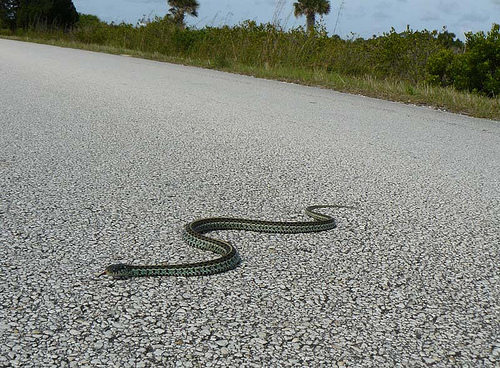
\includegraphics[trim={36mm 10mm 32mm 10mm},clip, width=\sizeP\textwidth]{fig/select/ILSVRC2012_val_00000006.JPEG}&
	\fig[\sizeS]{select/ILSVRC2012_val_00000006JPEG_vgg_GradCAM_vis.png} &
	\fig[\sizeS]{select/ILSVRC2012_val_00000006JPEG_vgg_GradCAMPlusPlus_vis.png} &
	\fig[\sizeS]{select/ILSVRC2012_val_00000006JPEG_vgg_ScoreCAM_vis.png} &
	\fig[\sizeS]{select/ILSVRC2012_val_00000006JPEG_vgg_AblationCAM_vis.png} &
	\fig[\sizeS]{select/ILSVRC2012_val_00000006JPEG_vgg_XGradCAM_vis.png} &
	\fig[\sizeS]{select/ILSVRC2012_val_00000006JPEG_vgg_versionP0_vis.png}  \\

	\rotatebox{90}{~Tricycle} &
	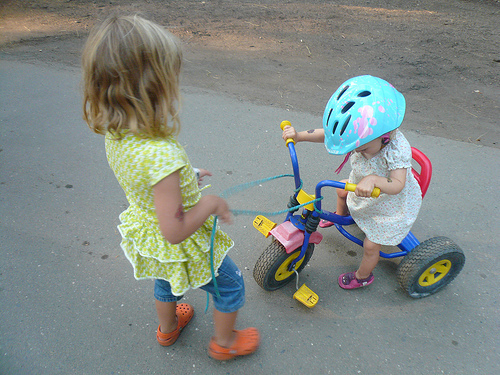
\includegraphics[trim={28mm 10mm 39mm 10mm},clip, width=\sizeP\textwidth]{fig/select/ILSVRC2012_val_00000069.JPEG}&
	\fig[\sizeS]{select/ILSVRC2012_val_00000069JPEG_vgg_GradCAM_vis.png} &
	\fig[\sizeS]{select/ILSVRC2012_val_00000069JPEG_vgg_GradCAMPlusPlus_vis.png} &
	\fig[\sizeS]{select/ILSVRC2012_val_00000069JPEG_vgg_ScoreCAM_vis.png} &
	\fig[\sizeS]{select/ILSVRC2012_val_00000069JPEG_vgg_AblationCAM_vis.png} &
	\fig[\sizeS]{select/ILSVRC2012_val_00000069JPEG_vgg_XGradCAM_vis.png} &
	\fig[\sizeS]{select/ILSVRC2012_val_00000069JPEG_vgg_versionP0_vis.png}  \\

	\rotatebox{90}{~Pneumonia} &
	\fig[\sizeS]{medical/chest_VGG16_GradCAM_1_img.png} &
	\fig[\sizeS]{medical/chest_VGG16_GradCAM_1_vis.png} &
	\fig[\sizeS]{medical/chest_VGG16_GradCAMPlusPlus_1_vis.png} &
	\fig[\sizeS]{medical/chest_VGG16_ScoreCAM_1_vis.png} &
	\fig[\sizeS]{medical/chest_VGG16_AblationCAM_1_vis.png} &
	\fig[\sizeS]{medical/chest_VGG16_XGradCAM_1_vis.png} &
	\fig[\sizeS]{medical/chest_VGG16_OptCAM_plain_1_vis.png}  \\


	\rotatebox{90}{~Pylorus} &
	\fig[\sizeS]{medical/kvasir_Resnet50_GradCAM_3_img.png} &
	\fig[\sizeS]{medical/kvasir_VGG16_GradCAM_3_vis.png} &
	\fig[\sizeS]{medical/kvasir_VGG16_GradCAMPlusPlus_3_vis.png} &
	\fig[\sizeS]{medical/kvasir_VGG16_ScoreCAM_3_vis.png} &
	\fig[\sizeS]{medical/kvasir_VGG16_AblationCAM_3_vis.png} &
	\fig[\sizeS]{medical/kvasir_VGG16_XGradCAM_3_vis.png} &
	\fig[\sizeS]{medical/kvasir_VGG16_OptCAM_plain_3_vis.png}  \\

\end{tabular}
\caption{Saliency maps obtained by different methods for ImageNet (top two rows), Chest X-ray (row 3) and Kvasir (row 4) with VGG. \iavr{Ground truth class shown on the left of the input image.}}
\label{fig:vis-in-chest-n-kvasir-resnet}
% \vspace{-0.4cm}
\end{figure*}